% Options for packages loaded elsewhere
\PassOptionsToPackage{unicode}{hyperref}
\PassOptionsToPackage{hyphens}{url}
%
\documentclass[
]{article}
\usepackage{amsmath,amssymb}
\usepackage{iftex}
\ifPDFTeX
  \usepackage[T1]{fontenc}
  \usepackage[utf8]{inputenc}
  \usepackage{textcomp} % provide euro and other symbols
\else % if luatex or xetex
  \usepackage{unicode-math} % this also loads fontspec
  \defaultfontfeatures{Scale=MatchLowercase}
  \defaultfontfeatures[\rmfamily]{Ligatures=TeX,Scale=1}
\fi
\usepackage{lmodern}
\ifPDFTeX\else
  % xetex/luatex font selection
\fi
% Use upquote if available, for straight quotes in verbatim environments
\IfFileExists{upquote.sty}{\usepackage{upquote}}{}
\IfFileExists{microtype.sty}{% use microtype if available
  \usepackage[]{microtype}
  \UseMicrotypeSet[protrusion]{basicmath} % disable protrusion for tt fonts
}{}
\makeatletter
\@ifundefined{KOMAClassName}{% if non-KOMA class
  \IfFileExists{parskip.sty}{%
    \usepackage{parskip}
  }{% else
    \setlength{\parindent}{0pt}
    \setlength{\parskip}{6pt plus 2pt minus 1pt}}
}{% if KOMA class
  \KOMAoptions{parskip=half}}
\makeatother
\usepackage{xcolor}
\usepackage[margin=1in]{geometry}
\usepackage{color}
\usepackage{fancyvrb}
\newcommand{\VerbBar}{|}
\newcommand{\VERB}{\Verb[commandchars=\\\{\}]}
\DefineVerbatimEnvironment{Highlighting}{Verbatim}{commandchars=\\\{\}}
% Add ',fontsize=\small' for more characters per line
\usepackage{framed}
\definecolor{shadecolor}{RGB}{248,248,248}
\newenvironment{Shaded}{\begin{snugshade}}{\end{snugshade}}
\newcommand{\AlertTok}[1]{\textcolor[rgb]{0.94,0.16,0.16}{#1}}
\newcommand{\AnnotationTok}[1]{\textcolor[rgb]{0.56,0.35,0.01}{\textbf{\textit{#1}}}}
\newcommand{\AttributeTok}[1]{\textcolor[rgb]{0.13,0.29,0.53}{#1}}
\newcommand{\BaseNTok}[1]{\textcolor[rgb]{0.00,0.00,0.81}{#1}}
\newcommand{\BuiltInTok}[1]{#1}
\newcommand{\CharTok}[1]{\textcolor[rgb]{0.31,0.60,0.02}{#1}}
\newcommand{\CommentTok}[1]{\textcolor[rgb]{0.56,0.35,0.01}{\textit{#1}}}
\newcommand{\CommentVarTok}[1]{\textcolor[rgb]{0.56,0.35,0.01}{\textbf{\textit{#1}}}}
\newcommand{\ConstantTok}[1]{\textcolor[rgb]{0.56,0.35,0.01}{#1}}
\newcommand{\ControlFlowTok}[1]{\textcolor[rgb]{0.13,0.29,0.53}{\textbf{#1}}}
\newcommand{\DataTypeTok}[1]{\textcolor[rgb]{0.13,0.29,0.53}{#1}}
\newcommand{\DecValTok}[1]{\textcolor[rgb]{0.00,0.00,0.81}{#1}}
\newcommand{\DocumentationTok}[1]{\textcolor[rgb]{0.56,0.35,0.01}{\textbf{\textit{#1}}}}
\newcommand{\ErrorTok}[1]{\textcolor[rgb]{0.64,0.00,0.00}{\textbf{#1}}}
\newcommand{\ExtensionTok}[1]{#1}
\newcommand{\FloatTok}[1]{\textcolor[rgb]{0.00,0.00,0.81}{#1}}
\newcommand{\FunctionTok}[1]{\textcolor[rgb]{0.13,0.29,0.53}{\textbf{#1}}}
\newcommand{\ImportTok}[1]{#1}
\newcommand{\InformationTok}[1]{\textcolor[rgb]{0.56,0.35,0.01}{\textbf{\textit{#1}}}}
\newcommand{\KeywordTok}[1]{\textcolor[rgb]{0.13,0.29,0.53}{\textbf{#1}}}
\newcommand{\NormalTok}[1]{#1}
\newcommand{\OperatorTok}[1]{\textcolor[rgb]{0.81,0.36,0.00}{\textbf{#1}}}
\newcommand{\OtherTok}[1]{\textcolor[rgb]{0.56,0.35,0.01}{#1}}
\newcommand{\PreprocessorTok}[1]{\textcolor[rgb]{0.56,0.35,0.01}{\textit{#1}}}
\newcommand{\RegionMarkerTok}[1]{#1}
\newcommand{\SpecialCharTok}[1]{\textcolor[rgb]{0.81,0.36,0.00}{\textbf{#1}}}
\newcommand{\SpecialStringTok}[1]{\textcolor[rgb]{0.31,0.60,0.02}{#1}}
\newcommand{\StringTok}[1]{\textcolor[rgb]{0.31,0.60,0.02}{#1}}
\newcommand{\VariableTok}[1]{\textcolor[rgb]{0.00,0.00,0.00}{#1}}
\newcommand{\VerbatimStringTok}[1]{\textcolor[rgb]{0.31,0.60,0.02}{#1}}
\newcommand{\WarningTok}[1]{\textcolor[rgb]{0.56,0.35,0.01}{\textbf{\textit{#1}}}}
\usepackage{graphicx}
\makeatletter
\def\maxwidth{\ifdim\Gin@nat@width>\linewidth\linewidth\else\Gin@nat@width\fi}
\def\maxheight{\ifdim\Gin@nat@height>\textheight\textheight\else\Gin@nat@height\fi}
\makeatother
% Scale images if necessary, so that they will not overflow the page
% margins by default, and it is still possible to overwrite the defaults
% using explicit options in \includegraphics[width, height, ...]{}
\setkeys{Gin}{width=\maxwidth,height=\maxheight,keepaspectratio}
% Set default figure placement to htbp
\makeatletter
\def\fps@figure{htbp}
\makeatother
\setlength{\emergencystretch}{3em} % prevent overfull lines
\providecommand{\tightlist}{%
  \setlength{\itemsep}{0pt}\setlength{\parskip}{0pt}}
\setcounter{secnumdepth}{-\maxdimen} % remove section numbering
\ifLuaTeX
  \usepackage{selnolig}  % disable illegal ligatures
\fi
\usepackage{bookmark}
\IfFileExists{xurl.sty}{\usepackage{xurl}}{} % add URL line breaks if available
\urlstyle{same}
\hypersetup{
  pdftitle={Creating images with R},
  pdfauthor={Anish Hota},
  hidelinks,
  pdfcreator={LaTeX via pandoc}}

\title{Creating images with R}
\usepackage{etoolbox}
\makeatletter
\providecommand{\subtitle}[1]{% add subtitle to \maketitle
  \apptocmd{\@title}{\par {\large #1 \par}}{}{}
}
\makeatother
\subtitle{My Car}
\author{Anish Hota}
\date{}

\begin{document}
\maketitle

\begin{Shaded}
\begin{Highlighting}[]
\NormalTok{body \{}\KeywordTok{font{-}weight}\CharTok{:} \DecValTok{bold}\NormalTok{\}}
\NormalTok{h1\{}\KeywordTok{background{-}color}\CharTok{:}\NormalTok{ \#}\ConstantTok{\#FFA500}\NormalTok{\}}
\NormalTok{p\{}\KeywordTok{color}\CharTok{:}\ConstantTok{\#0000FF}\NormalTok{\}}
\end{Highlighting}
\end{Shaded}

\subsection{Project requirements}\label{project-requirements}

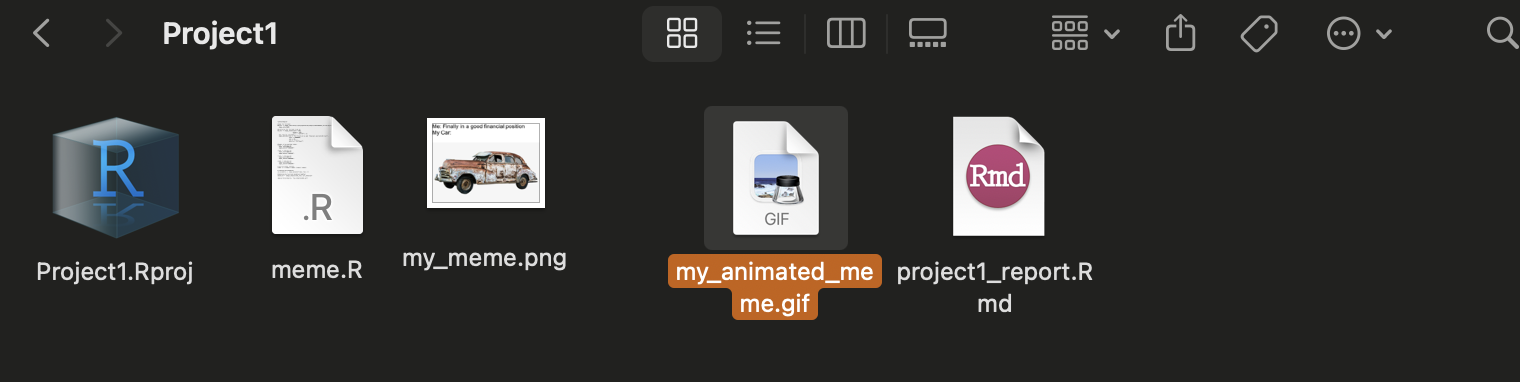
\includegraphics{/Users/anish/Desktop/stats220/Project1/Screenshot.png}
\href{https://github.com/ahot228/stats220}{My Github stats220c repo}
\#\# Inspo meme
\includegraphics{https://preview.redd.it/something-always-has-to-go-wrong-with-it-v0-g1xbe9pwkg3d1.jpeg?width=640&crop=smart&auto=webp&s=d349bc34bdbad6b7ae854915a1177d5fd426f84f}

\subsection{My meme}\label{my-meme}


\includegraphics{/Users/anish/Desktop/stats220/Project1/my_meme.png} I
just changed the image of this meme as the other image I feel didn't
make as much sense as this one does. \#\# My animated meme
\includegraphics{/Users/anish/Desktop/stats220/Project1/my_animated_meme.gif}

\subsection{Creativity}\label{creativity}

My project demonstrates creativity as I have use different ideas than
the ones that were used in the labs. For example my animated GIF I used
image\_composite in order to allow the text and GIF to work at the same
time. I also made the text a background instead of stack the two with
append. \#\# Learning reflection I learned that the magick package is a
very useful tool in order to make and produce memes that we see all the
time. It is also very easy to use and understand and is able to present
images and text very well. I liked that we were able to created little
animations using just code and how simple and efficient the R coding was
able to do this. I am excited to see how many different things we can
code using R and how we can utilize html and markdown files to present
different and cool ideas. I would love to learn more coding and more
innovative ideas that can help different aspects of the real world. \#\#
Appendix

Do not change, edit, or remove the \texttt{R} chunk included below.

If you are working within RStudio and within your Project1 RStudio
project (check the top right-hand corner says ``Project1''), then the
code from the \texttt{meme.R} script will be displayed below.

This code needs to be visible for your project to be marked
appropriately, as some of the criteria are based on this code being
submitted.

\begin{Shaded}
\begin{Highlighting}[]
\FunctionTok{library}\NormalTok{(magick)}

\CommentTok{\#image for the meme}
\NormalTok{bad\_car }\OtherTok{\textless{}{-}} \FunctionTok{image\_read}\NormalTok{(}\StringTok{"https://png.pngitem.com/pimgs/s/190{-}1905634\_old{-}car{-}png{-}transparent{-}png.png"}\NormalTok{) }\SpecialCharTok{\%\textgreater{}\%}
  \FunctionTok{image\_scale}\NormalTok{(}\DecValTok{500}\NormalTok{)}

\CommentTok{\#a white box for the text to go on}
\NormalTok{me\_text }\OtherTok{\textless{}{-}} \FunctionTok{image\_blank}\NormalTok{(}\AttributeTok{width =} \DecValTok{500}\NormalTok{,}
                       \AttributeTok{height =} \DecValTok{590}\NormalTok{,}
                       \AttributeTok{color =} \StringTok{"\#FFFFFF"}\NormalTok{) }\SpecialCharTok{\%\textgreater{}\%}
  \CommentTok{\#the text for the meme}
  \FunctionTok{image\_annotate}\NormalTok{(}\AttributeTok{text =} \StringTok{"Me: Finally in a good financial position}\SpecialCharTok{\textbackslash{}n}\StringTok{My Car:"}\NormalTok{,}
                 \AttributeTok{color =} \StringTok{"\#000000"}\NormalTok{,}
                 \AttributeTok{size =} \DecValTok{25}\NormalTok{,}
                 \AttributeTok{font =} \StringTok{"Arial"}\NormalTok{,}
                 \AttributeTok{gravity =} \StringTok{"northwest"}\NormalTok{)}

\CommentTok{\#frames of car getting bigger}
\NormalTok{frame1 }\OtherTok{\textless{}{-}}\NormalTok{ bad\_car }\SpecialCharTok{\%\textgreater{}\%}
  \FunctionTok{image\_scale}\NormalTok{(}\DecValTok{200}\NormalTok{)}\SpecialCharTok{\%\textgreater{}\%}
  \FunctionTok{image\_extent}\NormalTok{(}\StringTok{"500x500"}\NormalTok{)}

\NormalTok{frame2 }\OtherTok{\textless{}{-}}\NormalTok{ bad\_car }\SpecialCharTok{\%\textgreater{}\%}
  \FunctionTok{image\_scale}\NormalTok{(}\DecValTok{300}\NormalTok{)}\SpecialCharTok{\%\textgreater{}\%}
  \FunctionTok{image\_extent}\NormalTok{(}\StringTok{"500x500"}\NormalTok{)}

\NormalTok{frame3 }\OtherTok{\textless{}{-}}\NormalTok{ bad\_car }\SpecialCharTok{\%\textgreater{}\%}
  \FunctionTok{image\_scale}\NormalTok{(}\DecValTok{400}\NormalTok{)}\SpecialCharTok{\%\textgreater{}\%}
  \FunctionTok{image\_extent}\NormalTok{(}\StringTok{"500x500"}\NormalTok{)}

\NormalTok{frame4 }\OtherTok{\textless{}{-}}\NormalTok{ bad\_car }\SpecialCharTok{\%\textgreater{}\%}
  \FunctionTok{image\_scale}\NormalTok{(}\DecValTok{500}\NormalTok{)}\SpecialCharTok{\%\textgreater{}\%}
  \FunctionTok{image\_extent}\NormalTok{(}\StringTok{"500x500"}\NormalTok{)}

\CommentTok{\# putting frames together}
\NormalTok{frames }\OtherTok{\textless{}{-}} \FunctionTok{c}\NormalTok{(frame1, frame2, frame3, frame4)}

\CommentTok{\# creating the animation}
\NormalTok{car\_animation }\OtherTok{\textless{}{-}} \FunctionTok{image\_animate}\NormalTok{(frames, }\AttributeTok{fps =} \DecValTok{1}\NormalTok{)}

\CommentTok{\#combining the text and animation together}
\NormalTok{animation }\OtherTok{\textless{}{-}} \FunctionTok{image\_composite}\NormalTok{(me\_text, car\_animation)}

\FunctionTok{image\_write}\NormalTok{(animation, }\StringTok{"my\_animated\_meme.gif"}\NormalTok{)}
\end{Highlighting}
\end{Shaded}


\end{document}
